\documentclass[12pt]{article}
\usepackage[margin=1.05in]{geometry}                % See geometry.pdf to learn the layout options. There are lots.
\geometry{letterpaper}                   % ... or a4paper or a5paper or ... 
%\geometry{landscape}                % Activate for for rotated page geometry
%\usepackage[parfill]{parskip}    % Activate to begin paragraphs with an empty line rather than an indent

%\usepackage{mathptmx}
\usepackage[superscript,biblabel]{cite}
\usepackage{graphicx}
\usepackage{amssymb}
\usepackage{epstopdf}
\usepackage{changepage}
\usepackage{setspace}
\usepackage{amsthm}
\usepackage{amsmath}
\usepackage{braket}
\usepackage{mathtools}
\usepackage{algorithm}
\usepackage{algpseudocode}
\usepackage{listings}
\usepackage{subcaption}
\usepackage{caption}
\usepackage{tabularx}  % for 'tabularx' environment and 'X' column type
\usepackage{ragged2e}  % for '\RaggedRight' macro (allows hyphenation)
\newcolumntype{Y}{>{\RaggedRight\arraybackslash}X} 
\usepackage{booktabs}  % for \toprule, \midrule, and \bottomrule macros 
\makeatletter
\renewcommand{\ALG@beginalgorithmic}{\small}
\makeatother

\makeatletter
\setlength{\@fpbot}{0pt}
\makeatother

\usepackage[utf8]{inputenc}
\usepackage[english]{babel}
\newtheorem{theorem}{Theorem}[section]
\newtheorem{lemma}[theorem]{Lemma}

\DeclareGraphicsRule{.tif}{png}{.png}{`convert #1 `dirname #1`/`basename #1 .tif`.png}
\newcommand\permute[2][n]{\prescript{#1\mkern-2.5mu}{}P_{#2}}




\begin{document}

\title{An Average Case Complexity Speedup for the Graph Isomorphism Problem}
\date{}                                           % Activate to display a given date or no date
\maketitle
\doublespacing
%\section{}
%\subsection{}
\abstract{\noindent The Graph Isomorphism Problem is a well-known open problem in Computer Science. Currently, researchers Babai and Luks\cite{7} hold the record for the fastest computational complexity of $2^{O\sqrt{n}log^2n}$}. In this paper, we introduce a novel approach to the problem, in which we limit the total number of adjacency matrices that may act as candidates for isomorphism. In the average case, our algorithm provides a speedup from the algorithm of Babai and Luks\cite{7} , and potentially introduces a new approach to the Isomorphism problem, which can lead to further progress and a possible polynomial-time algorithmic solution.
\clearpage

\section[Theory]{Theoretical Approach}
\subsection{The Graph Isomorphism Problem}
The graph isomorphism problem is defined as follows\cite{1}  :


\begin{adjustwidth}{3em}{0pt}
\singlespace
Two graphs $G$ and $G'$ are determined to be isomorphic if and only if there exists a permutation of the vertices of $G$ which preserves vertex adjacency and transforms $G \rightarrow G'$. Given two $N$-vertex graphs $G$ and $G'$, determine in polynomial time whether they are isomorphic to one another.
\end{adjustwidth}
\doublespace

While seemingly simple on the surface, this problem has eluded a proof since before 1970\cite{3} . This problem is of particular importance because of its far-reaching multi-field consequences, such as identification in the tertiary structure of proteins\cite{2} . Many attempts have been made to solve this problem, yet there is not one definite solution \cite{1,3,4,5,6,7} . In this section, we will discuss a systematic method to define a graph $G$ in matrix form, and then describe a mathematical model to simplify the problem at hand.

A graph $A$ with $n$ vertices, labelled $1\ldots i\ldots j \ldots n$, can be described by a $n \times n$ matrix $A$, where $A_{i,j}\in\{0,1\}$. This matrix, called the \textit{adjacency matrix}\cite{1} , describes the adjacency of vertex $i$ with vertex $j$. If vertex $i$ is adjacent to vertex $j$(\textit{i.e} there is an edge between vertices $i$ and $j$), then $A_{i,j} = 1$. Inversely, if vertex $i$ is not adjacent to vertex $j$, then $A_{i,j} = 0$. Since a vertex can not be adjacent to itself, when $i=j$, then $A_{i,j} = 0$. Therefore, the diagonal of matrix $A$ is composed of $A_{m,m} = 0$ for $m<n$.

If vertex $i$ is adjacent to vertex $j$, it is trivial to observe that vertex $j$ must also be adjacent to vertex $i$, by the same edge. From this fact, we have $A_{i,j} = A_{j,i}$ for all positive $i,j \le n$, and by definition $A$ is a symmetric matrix.

A permutation matrix $\sigma$ is defined as a $n \times n$ matrix in which each row $i$ and column $j$ contains exactly a single $1$, and all other entries are $0$. A permutation matrix can be visualized as reordering either the rows or columns of a matrix.


\subsection{A Mathematical Description}


Let graph $G$ have adjacency matrix $A$, and graph $G'$ have adjacency matrix $A'$. From the problem statement, we can observe that $G$ is isomorphic to $G'$ if and only if a permutation matrix $\sigma$ satisfies the following\cite{1} :

\begin{equation}
A' = \sigma A \sigma^T
\end{equation}

Our task now is to find a computationally simple method to find the $\sigma$ satisfying the condition above. In order to do this, we will simplify the equation $(1)$.

Because the inverse of a permutation is exactly equal to its transpose, we can redefine $(1)$ as:

\[A' = \sigma A \sigma^{-1}\]
\[A' \sigma = \sigma A \sigma^{-1} \sigma\]
\begin{equation}
A' \sigma = \sigma A
\end{equation}

One of the many remarkable properties of a permutation matrix(from which it derives its name) $P$ is that for any matrix $G$ which multiplies $P$ such that $PG = G'$, $G'$ is simply a reordering of the columns of $G$. Similarly, if the multiplication is rewritten such that $GP = G'$, due to the non commutativity of matrices, then $G'$ is a reordering of the rows of $G$. This property is trivial to prove, as permutation matrices by definition lend themselves to these properties.

\subsection{Matrix dependencies}

From (2), we gather that the graphs of two adjacency matrices $A$ and $A'$ are isomorphic iff there exists some permutation $\sigma$ that can be performed upon the rows of $A$ and the columns of $A'$, or vice versa, such that $\sigma A = A' \sigma$. Let the notation $A_{\sigma[m]}$ be defined, for any $n \times n$ matrix $A$, as the position of the row vector $A_m$ after a permutation $\sigma$ has been performed on $A$, and $A_{\sigma(m)}$ be defined as the position of the column vector $A_m$ after a permutation $\sigma$ has been performed on $A$.

The reason that this problem proves to be so difficult is because there are about $n!$ different permutation matrices that are possible candidates for selection. Our task is, then, to reduce the number of possible matrices that we must test.

Since the same permutation $\sigma$ is being performed symmetrically on both $A$ and $A'$, we can notice that for any natural number $m<n$, $A_{\sigma[m]}$ and $A'_{\sigma(m)}$ must share some element, located at $A_{\sigma[m], \sigma(m)} = A'_{\sigma[m], \sigma(m)}$.


Let us now define the function $f$:
\begin{equation}
f(m,x) = A_{m,x} \oplus A'_{x,m}
\end{equation}
where $\oplus$ is defined as addition modulo $2$. For all numbers in the domain of this function, $f(m,x)$ will return:

 \begin{displaymath}
   f(m,x) = \left\{
     \begin{array}{lr}
       0 & A_{\sigma[m], \sigma(m)} = A'_{\sigma[m], \sigma(m)}\\
       1 & A_{\sigma[m], \sigma(m)} \neq A'_{\sigma[m], \sigma(m)}
     \end{array}
   \right.
\end{displaymath} 

Let us define a new array $A^*$ as:

\begin{equation}
A^*_{r,c} = f(r,c)
\end{equation}


\section{An Algorithmic Approach}
It is clear from the previous section that only zero values of $A^*$ can serve as 'points of intersection' between any row and column in $A \sigma$. However, in order for $A \sigma = \sigma A'$ to hold, the result of every intersection of row and column must agree with one another.

On average, the adjacency matrix will hold exactly $\frac{n^2}{2}$ zero elements, which are all evenly distributed across the matrix (with exception to the diagonal, which is always composed of zero elements). Because, in an average case, both $A$ and $A'$ follow these properties, we can assume that they will also hold true for $A^*$. Specifically, we can also conclude that, on average, every row and column of $A^*$ will also hold $\frac{n}{2}$ zero elements. Because only the average case is being observed, the parity of $n$ is irrelevant. We can also assume that the rows and columns of $A$ and $A'$ are independent of one another, and each element of each matrix on one side of the diagonal is randomly chosen independently; note that once one side of the diagonal has been set, the other side must be as well, since the matrices must be symmetric by definition.

\begin{lemma}
For all $m<n$, the number of valid rows which can serve as $A \sigma_{m}$ approaches $1$ as $m \to n.$
\end{lemma}
\begin{proof}
Let us primarily observe only the first row of $A^*$ in an average case. Since $A^*$ contains $\frac{n}{2}$ zero elements here, we can infer that there are exactly $\frac{n}{2}$ possible rows in $A$ which can compose the first row of $A \sigma$. Because all rows are equally valid, it is not clear which row may produce an isomorphism, so we must observe all rows equally. However, if row vector $A_{[m_1]}$ is chosen as the first row vector in $A \sigma$, then it also must be true that the column vector $A'_{(m_1)}$ must serve as the first column vector in $\sigma A' = A \sigma$, since the same permutation $\sigma$ is acting upon both matrices. Note that $A^*_{m_1, 0} = 0$.

We must now find a new row vector in $A$ to exist at $A \sigma_{[m_1]}$, let it be called $A_{m_2}$. Using the same argument as above, there are $\frac{n-1}{2}$(notice that $n-1$ is only on average; there is a $\frac{1}{2}$ chance that the row used previously could possibly be used to fill in the next row) row vectors in $A$ satisfying these conditions; in this case, $A^*_{m_2,m_1} = 0$. However, since the value of $A \sigma_{[0]}$ was already set, this new row placement must agree with the previous one; specifically, $A_{m_2, 0} = A'_{0, m_1}$. If this was not true, then the two row placements would disagree on the value of $A \sigma_{m_2, 0}$. 

Since both $A_{m_2, 0}$ and $A'_{0, m_1}$ were independent of one another and randomly chosen, we can assume that the equality $A_{m_2, 0} = A'_{0, m_1}$ is true only with a probability of $\frac{1}{2}$. Thus, the possible $A_{m_2}$ that satisfy the above conditions has been reduced to $\frac{n}{4}$.

We can apply this argument recursively. Let there be $m$ rows and columns already placed in $A \sigma$. Then, there are $\frac{n-m}{2}$ possible row vectors in $A$ which are candidates for the vacant row vector in $A \sigma$ in the average case. However, whichever row vector is chosen must agree with all other column vectors already placed; that is, if the rows and columns already placed are labelled $1 \dots m$, then $$\sum_{p=0}^{m} (A_{m+1, p} \oplus A'_{p,m+1}) = 0$$ where $\oplus$ is defined as addition modulo 2. However, each term in this summation will only be zero if $A_{m+1,p} = A'_{p,m+1}$, which in average case occurs with chance $\frac{1}{2}$. Thus, the chance that all terms in the sum will be zero has only a chance of $\frac{1}{2^m}$, which decreases exponentially in terms of $m$. Thus, as $m$ increases, the number of valid rows in position $m+1$ for $A \sigma$ decreases exponentially; this means that $$\lim_{m \to n} (\lceil\frac{n-m}{2^m}\rceil) = 1$$.
\end{proof}

Because of this lemma, the total number of rows we must check as a possible row for $A \sigma$ reduces to $\lceil\frac{n}{2}\rceil \times \lceil\frac{n}{4}\rceil \times \lceil\frac{n}{8}\rceil \dots$, or: 
$$\prod_{a=0}^{n-1} \lceil\frac{n-a}{2^a}\rceil$$
 As $n$ gets arbitrarily large, the $\pm 1$ difference in each product term greater than $1$ due to the ceiling function becomes negligible. Let us define $b$ as the first product term for which $\frac{n-b}{2^b} \leq 1$; for all product terms in which $a>b$, the product term becomes $1$, and in this case, the ceiling function is vastly important. Note that $b$ is roughly approximated to the lowest power of $2$ which divides $n$, or $\lfloor log_2 n \rfloor$. Thus, we may further reduce this expression to: 
 $$\prod_{a=0}^{n-1} \lceil\frac{n-a}{2^a}\rceil = \prod_{a=0}^{b} \lceil\frac{n-a}{2^a}\rceil \approx \prod_{a=0}^{b} \frac{n-a}{2^a}  = \frac{\permute{b+1}}{2^{1+2+ \dots +b}} $$
The power of $2$ is equivalent to $1 + 2 + \dots +b = \frac{b(b+1)}{2} = \frac{b^2}{2} + \frac{b}{2}$. However, as $n$ grows arbitrarily large, $b$ does as well, and this can be further reduced to simply $b^2$. The expression is then:
\begin{equation}
\frac{\permute{b+1}}{2^{1+2+ \dots +b}} \approx \frac{\permute{b+1}}{2^{b^2}} = \frac{n!}{2^{b^2} (n-b-1)!}
\end{equation}

Thus, in the average case, the number of possible matrices that this algorithm will require to be tested is approximately equal to $(5)$. The graph of $(5)$ between $n=0$ and $n=150$ is given in Appendix A; from this graph, we can infer that as $n$ gets arbitrarily large, $(5)$ begins to act linear.

The complete algorithm is given in Appendix B, in pseudocode, and in Appendix C, in the Python programming language.

The consequences of this algorithm are vast. Specifically, the number of possible matrices which can be produced from a permutation on $A$ and $A'$ have been drastically reduced from $n!$ to a function behaving almost linearly. While this algorithm only provides a speedup as the adjacency matrices is close to the average matrix of order $n$, this condition is true the majority of the time, and thus the algorithm proves useful in many situations. This algorithm does not solve the Graph Isomorphism Problem, but does provide an efficient attack at the problem in the average case.
\newpage

\section{Algorithm Application}

In this section, we will test the algorithm against some common graph categories and methods for creating random graphs, with $n = 9$. Although this is by no means an exhaustive search for a counterexample, and $n$ is not particularly large, we test a wide variety of graphs with different aspects, and a small $n$ allows for convenient display, as well as quick runtime. This section serves as a proof of concept rather than a thorough testing of the algorithm; more research may be necessary in this area. Additionally, since so few test cases are being performed, the speedup of the algorithm is not as pronounced; however, the validity of the algorithm is confirmed, and isomorphism detection is confirmed. Each section contains a brief description of the graph category or random method, followed by one pair of isomorphic graphs in the category, a graph not isomorphic to the first two. Each section will also define the runtime and result of the algorithm. All graphs were developed using the multiple Random Graph functions given in the Sage runtime environment, with probability 0.5. Isomorphisms were made by randomly permuting rows and columns of an adjacency matrix given from Sage.

The second part of this section tests graphs of order $n=10,50,100$, as well as data pertaining to runtime and efficiency of the algorithm. This section highlights the advantage of this algorithm, and implies the algorithm complexity.

All tests in this section were performed by a Macintosh MacBook Pro: Serial Number C2QN301YFG1H. The processor used was a 2.4 GHz Intel Core i7. All cases ran under the same conditions barring minor environmental fluctuations.

\newpage
\subsection{General Random Graph}
Perhaps the broadest category, this is simply a graph in which each edge between two vertices exists with probability $0.5$.
\begin{equation}
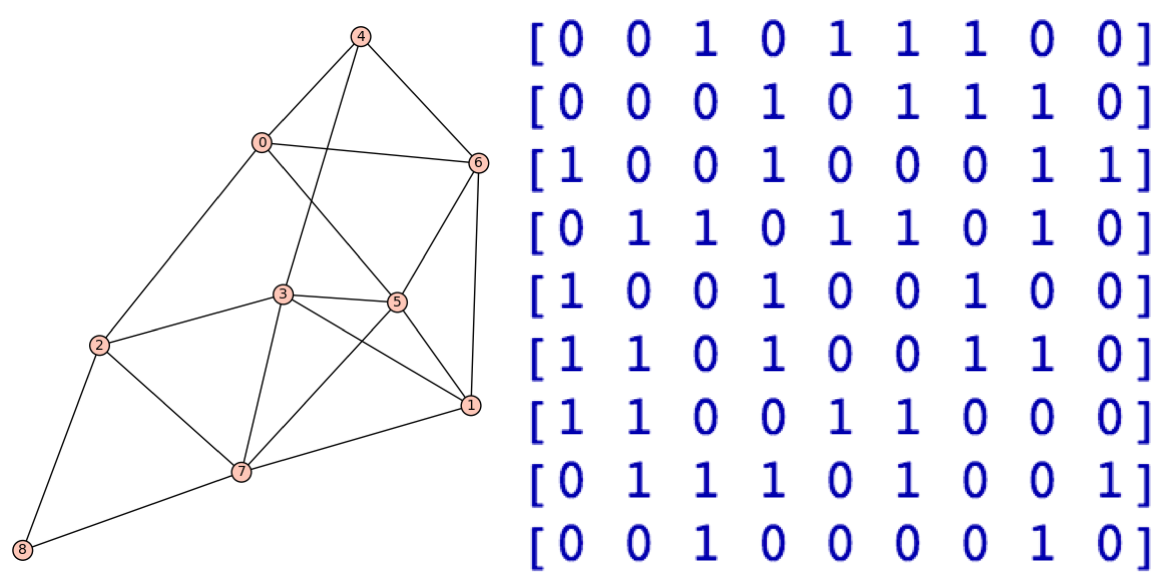
\includegraphics[width=200px,height=100px]{GNPIso1}
\end{equation}
\begin{equation}
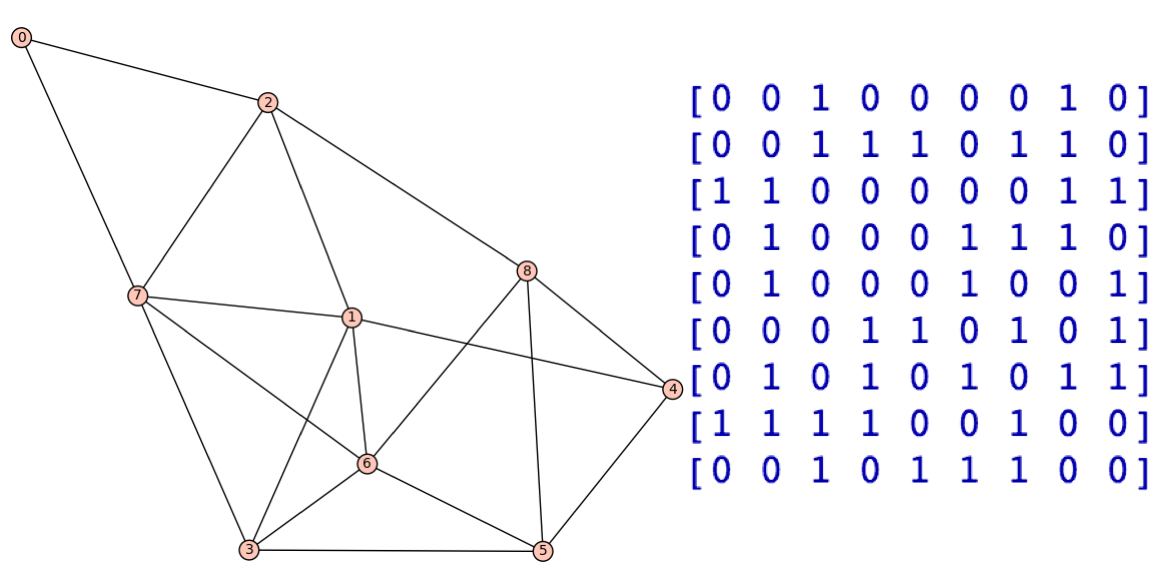
\includegraphics[width=200px,height=100px]{GNPIso2}
\end{equation}
\begin{equation}
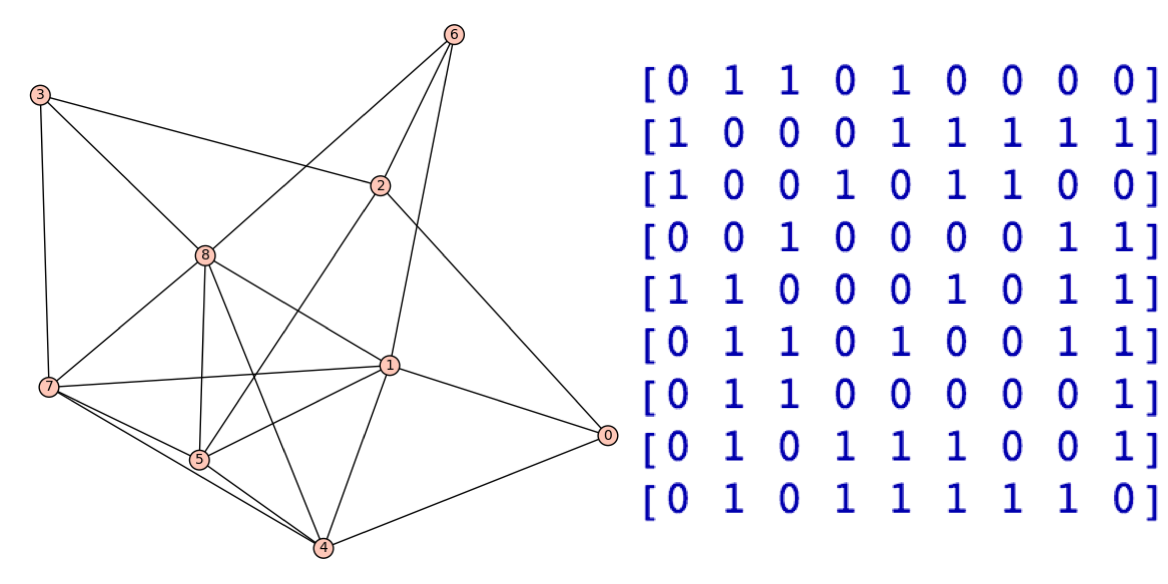
\includegraphics[width=200px,height=100px]{GNPNIso1}
\end{equation}

Graphs $6,7$ are isomorphic to one another; graph $8$ is not.

\begin{center}
    \begin{tabular}{ | l | l | l | p{5cm} |}
    \hline
    Graphs Tested & Permutation List Result & Runtime(s) & Expected Result? \\ \hline
    (6) (7) & [8, 3, 2, 1, 4, 6, 5, 7, 0] & 0.066 & Yes\\ \hline
    (6) (8) & No Isomorphism Found! & 0.1 &  Yes\\ \hline
    (7) (8) & No Isomorphism Found! & 0.088 & Yes \\
    \hline
    \end{tabular}
\end{center}

\newpage

\subsection{Bipartite Graphs}
A bipartite graph is a graph with vertices $V$ in which there exist two subsets $U$ and $T$ for which $U,T \subset V$, $U \cup T \cong V$, and $U \cap T \cong \varnothing$.

\begin{equation}
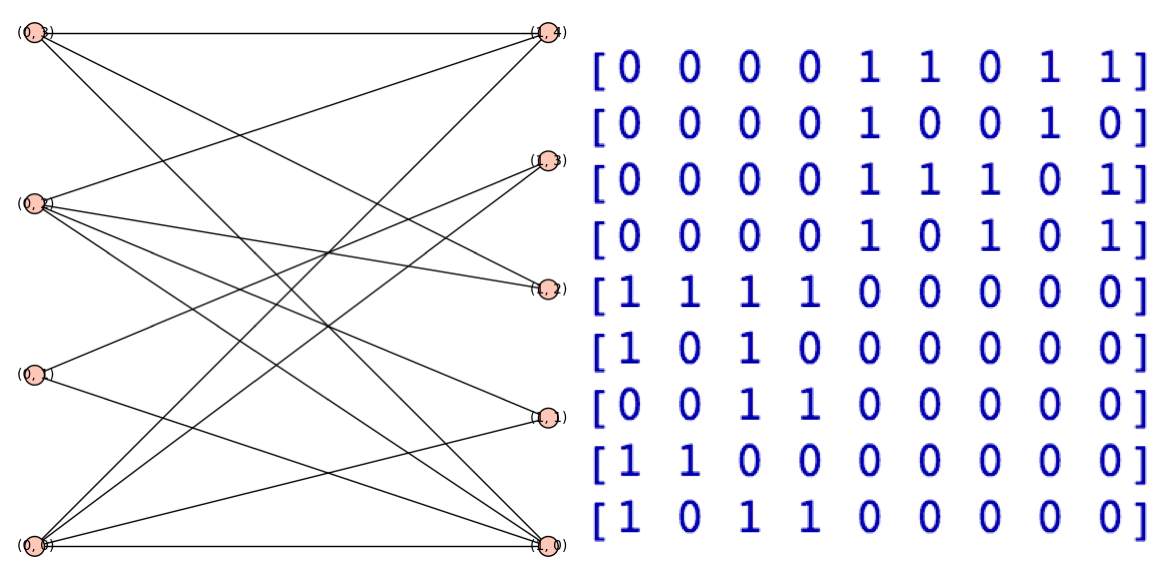
\includegraphics[width=200px,height=100px]{BipartiteIso1}
\end{equation}
\begin{equation}
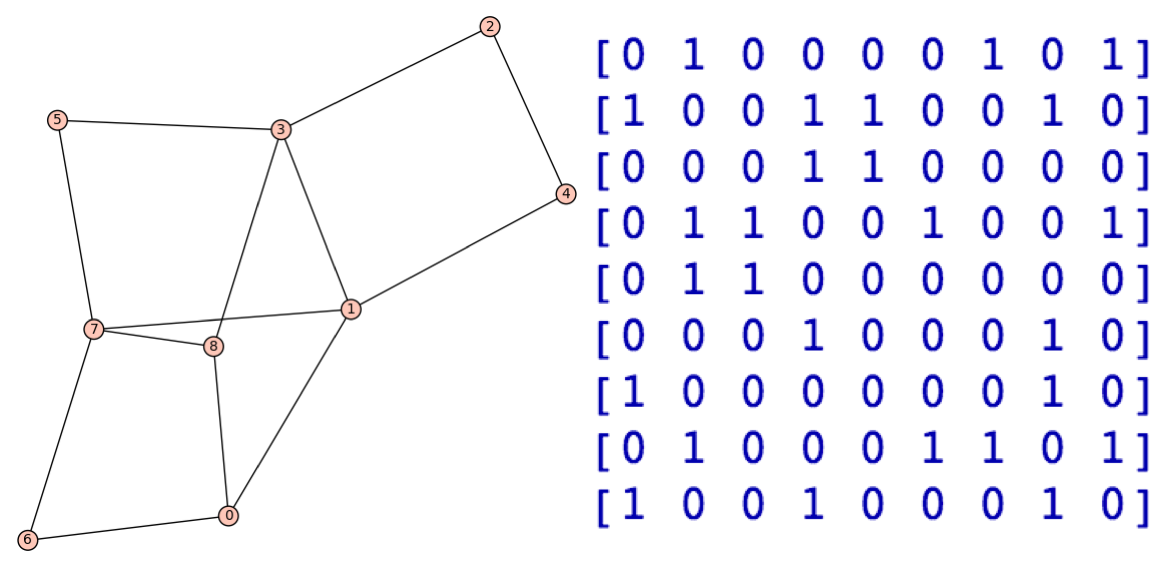
\includegraphics[width=200px,height=100px]{BipartiteIso2}
\end{equation}
\begin{equation}
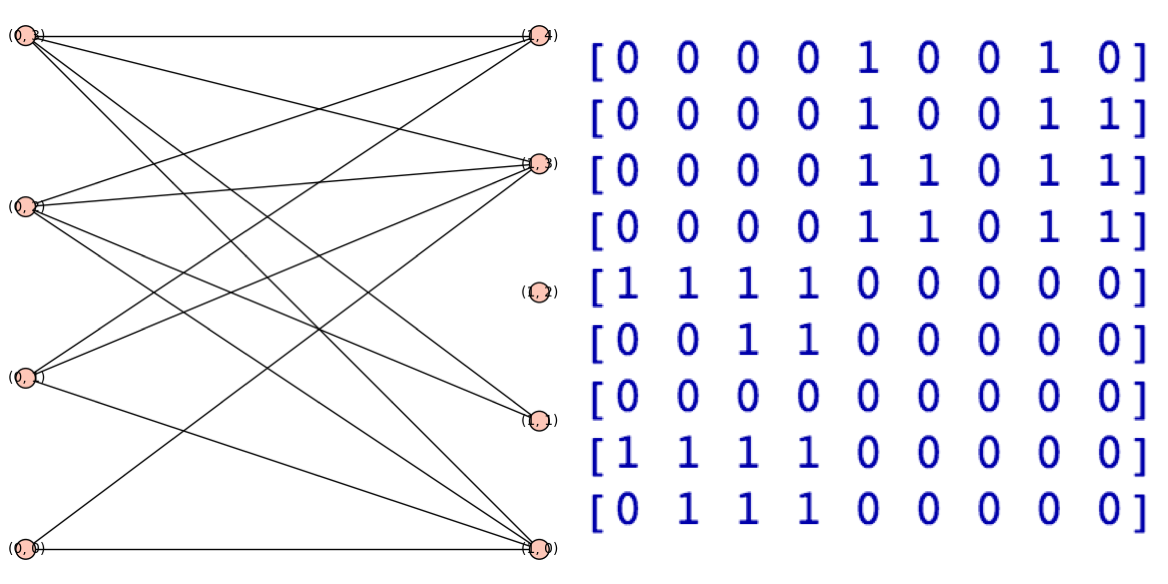
\includegraphics[width=200px,height=100px]{BipartiteNIso1}
\end{equation}

Graphs $9,10$ are isomorphic to one another; graph $11$ is not.

\begin{center}
    \begin{tabular}{ | l | l | l | p{5cm} |}
    \hline
    Graphs Tested & Permutation List Result & Runtime(s) & Expected Result? \\ \hline
    (9) (10) & [3, 4, 7, 0, 1, 5, 6, 2, 8] & 0.108 & Yes\\ \hline
    (9) (11) & No Isomorphism Found! & 0.122 &  Yes\\ \hline
    (10) (11) & No Isomorphism Found! & 0.073 & Yes \\
    \hline
    \end{tabular}
\end{center}

\newpage

\subsection{Barabasi Albert Graph Randomization} 
We begin with a graph with m vertices and no edges, and add new vertices each with m edges to existing vertices, preferably with high degree.

\begin{equation}
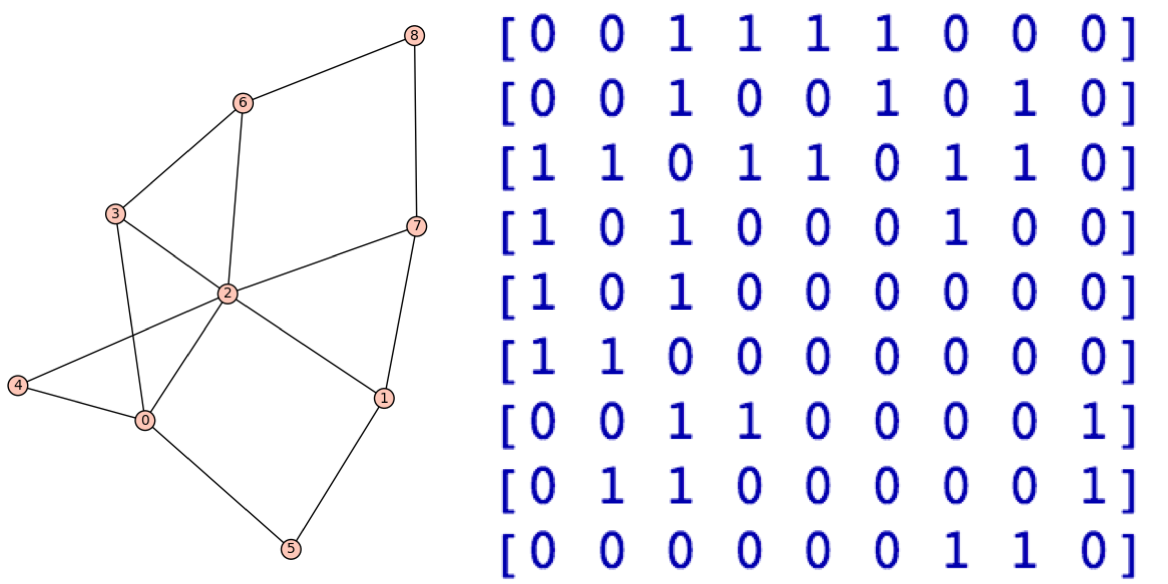
\includegraphics[width=200px,height=100px]{RBAIso1}
\end{equation}
\begin{equation}
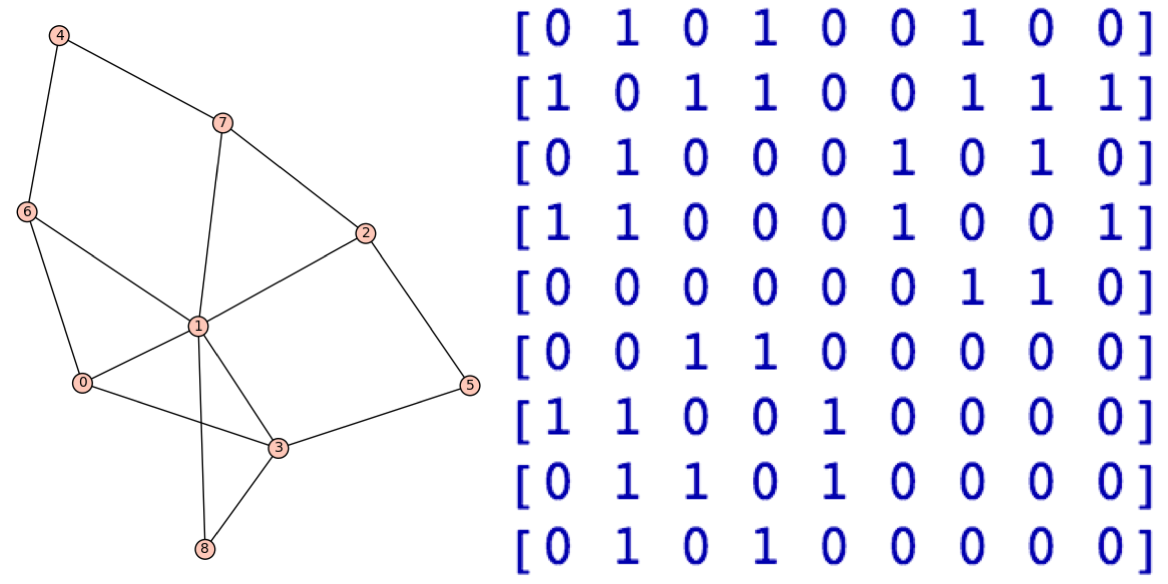
\includegraphics[width=200px,height=100px]{RBAIso2}
\end{equation}
\begin{equation}
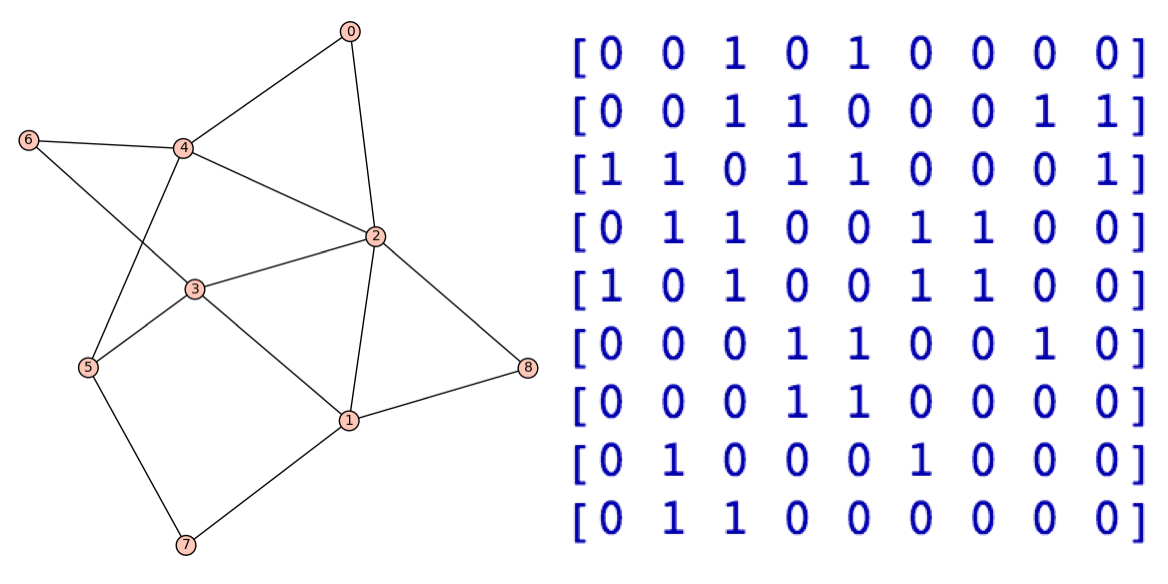
\includegraphics[width=200px,height=100px]{RBANIso1}
\end{equation}

Graphs $12,13$ are isomorphic to one another; graph $14$ is not.
\begin{center}
    \begin{tabular}{ | l | l | l | p{5cm} |}
    \hline
    Graphs Tested & Permutation List Result & Runtime(s) & Expected Result? \\ \hline
    (12) (13) & [3, 2, 1, 0, 8, 5, 6, 7, 4] & 0.068 & Yes\\ \hline
    (12) (14) & No Isomorphism Found! & 0.065 &  Yes\\ \hline
    (13) (14) & No Isomorphism Found! & 0.068 & Yes \\
    \hline
    \end{tabular}
\end{center}

\newpage

\subsection{Holme Kim Graph Randomization}
Essentially, this algorithm is the Barabasi Albert Graph Randomization algorithm but with one extra feature; for each random edge, there is an additional probability that the vertex will form another adjacency to form a triangle. 

\begin{equation}
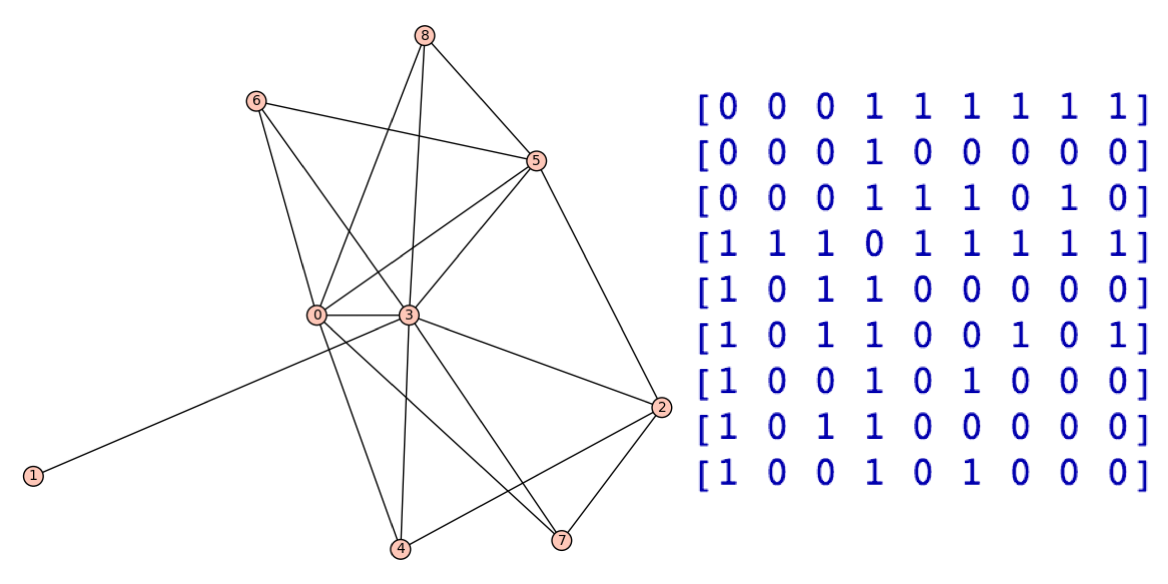
\includegraphics[width=200px,height=100px]{HKIso1}
\end{equation}
\begin{equation}
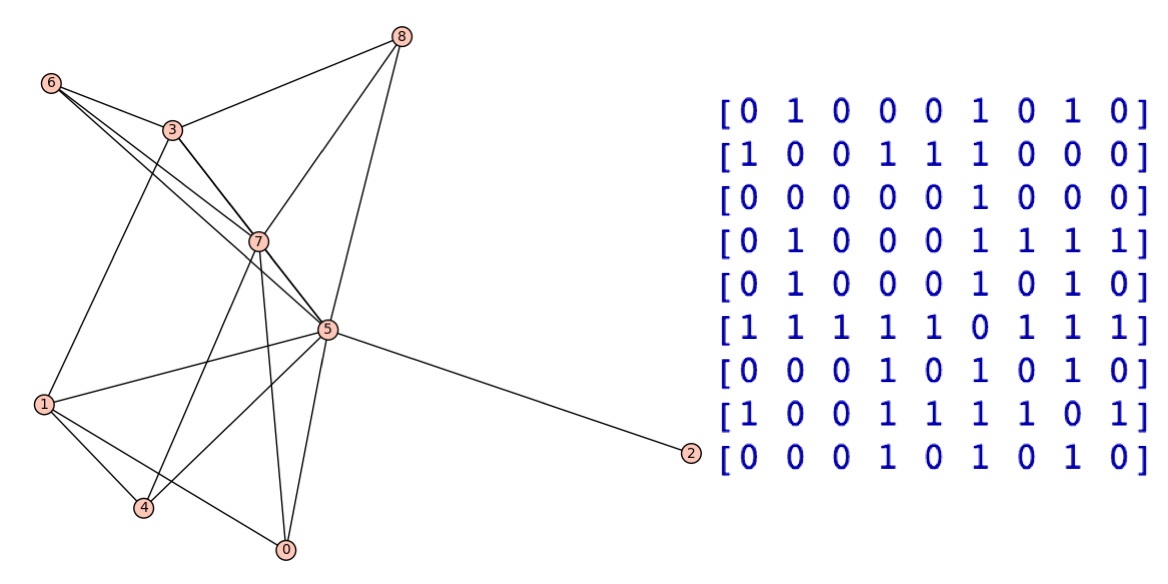
\includegraphics[width=200px,height=100px]{HKIso2}
\end{equation}
\begin{equation}
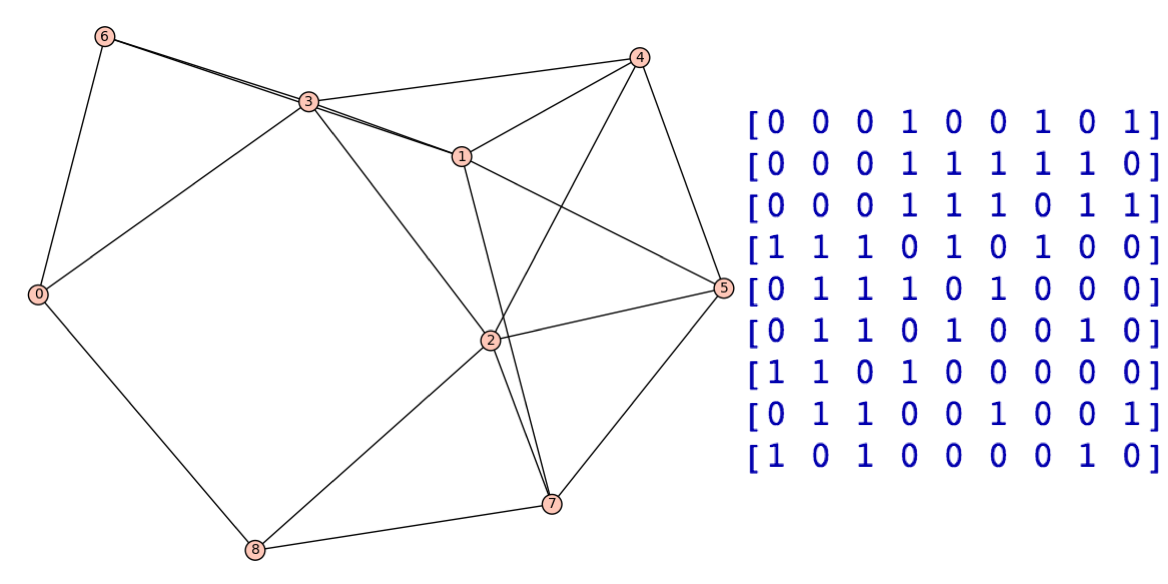
\includegraphics[width=200px,height=100px]{HKNIso1}
\end{equation}

Graphs $15,16$ are isomorphic to one another; graph $17$ is not.
\begin{center}
    \begin{tabular}{ | l | l | l | p{5cm} |}
    \hline
    Graphs Tested & Permutation List Result & Runtime(s) & Expected Result? \\ \hline
    (15) (16) & [7, 2, 1, 5, 4, 3, 6\footnotemark, 0, 6] & 0.067 & Yes\\ \hline
    (15) (17) & No Isomorphism Found! & 0.108 &  Yes\\ \hline
    (16) (17) & No Isomorphism Found! & 0.106 & Yes \\
    \hline
    \end{tabular}
\end{center}
\footnotetext{Note: There is a repeating 6 in the permutation list for Holme Kim Randomization Isomorphisms. This is because row 6 and row 8 of $(15)$ are exactly congruent; the same correct result is obtained.}
\newpage
\subsection{Larger $n$}
Due to space restraints, the adjacency matrices of the graphs below will not be given. However, the runtime and matrix order may provide the reader insight to how the algorithm deals with larger inputs. These graphs were made by using General Random Graph method highlighted in section $3.1$
First, we tested two graphs which were created by shifting some rows and columns randomly in the first graph to create the second one. Next, we changed 5 non diagonal entries in the adjacency matrix of the second graph, chosen randomly, to assure that the algorithm detected non isomorphism as well; this "incorrect" matrix will be denoted with a ' next to the name of the original matrix. Larger $n>100$ were difficult to test due to computational constraints set by the device used. The results for $n = 10, 50, 100$ are shown below.
\begin{center}
    \begin{tabular}{ | l | l p{5cm} |}
   \hline
    Graphs Tested & Runtime(s) \\  \hline 
    (18) (19) & & 0.181\\ \hline
    (18) (19') & & 0.114\\ \hline
    (20) (21) & & 0.5\\ \hline
    (20) (21') & & 0.79\\ \hline
    (22) (23) & & 8.021\\ \hline
    (22) (23') & & 10.31\\ \hline
    \hline
    \end{tabular}
\end{center}


\begin{figure}[b]
\centering
\begin{subfigure}{.5\textwidth}
  \centering
  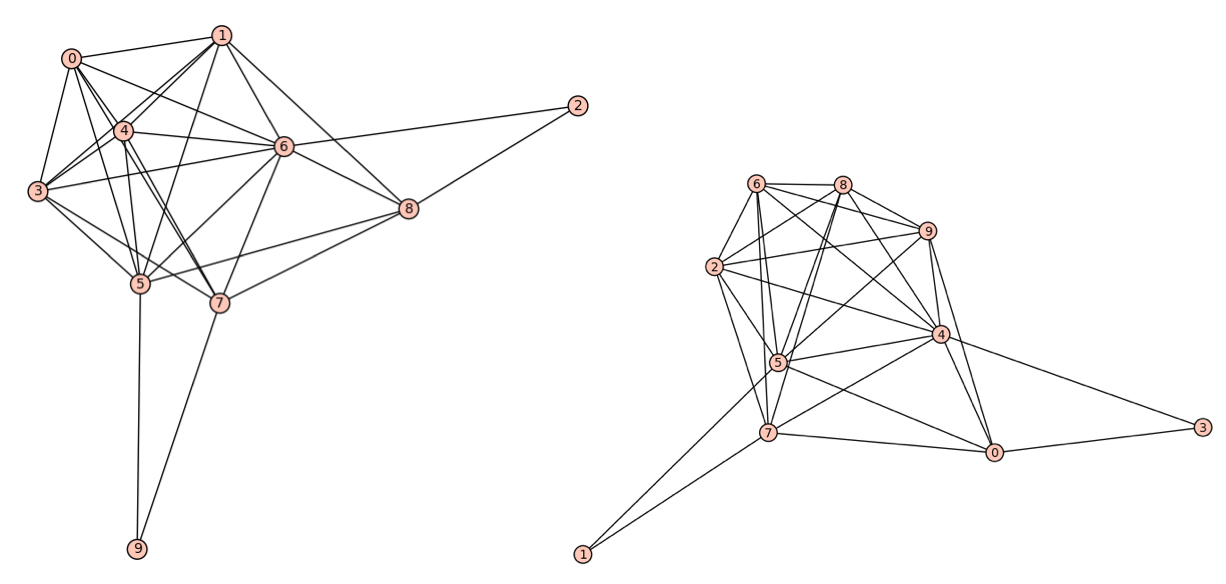
\includegraphics[width=.55\linewidth]{LargeN10}
  \caption{$n=10$}
  \label{fig:sub1}
\end{subfigure}%
\begin{subfigure}{.5\textwidth}
  \centering
  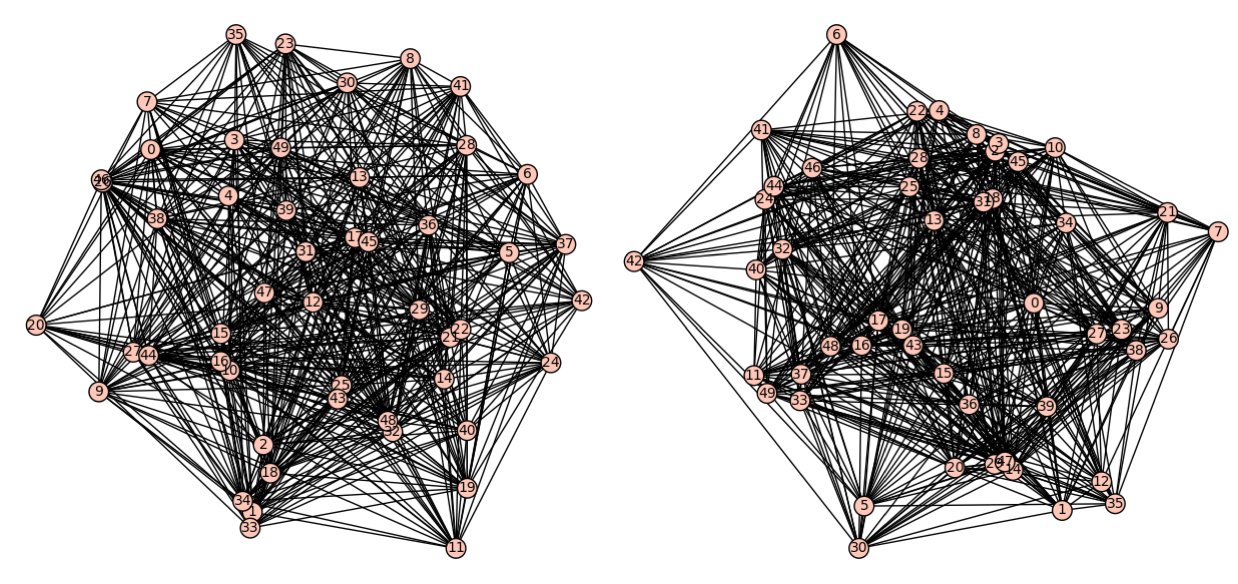
\includegraphics[width=.55\linewidth]{LargeN50}
  \caption{$n=50$}
  \label{fig:sub2}
\end{subfigure}
\begin{subfigure}{.5\textwidth}
  \centering
  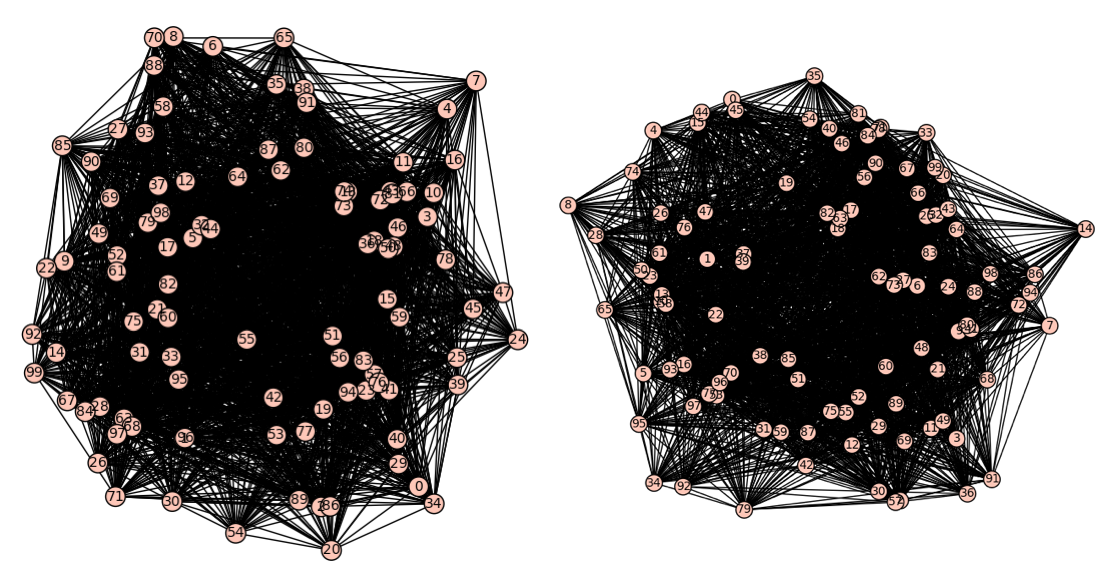
\includegraphics[width=.55\linewidth]{LargeN100}
  \caption{$n=100$}
  \label{fig:sub2}
\end{subfigure}
\caption{Graphs with larger $n$}
\label{fig:Graphs}
\end{figure}

\section{Conclusion}
This algorithm provides a large advantage over those commonly used today. While this algorithm only proves a speedup in the average case, its applications in industry and research alike are vast. By limiting the number of possible matrices that can prove to be an isomorphism from $n!$ to only 
$\frac{n!}{2^{b^2} (n-b-1)!}$, where $b = log_2 n$, this algorithm simplifies the graph isomorphism to a search of a list of trivial size in the average case. 

One major application of this algorithm is in definition and classification of protein structure\cite{2} . As seen from \textbf{Section 3.5}, this algorithm is capable of parsing through large adjacency matrices and finding an isomorphism in a reasonable time. Proteins whose structures otherwise seem very complex and completely dissimilar may prove to be the exact same protein; this revelation may lead to further advances in both biology and chemistry due to its ability to distinguish molecular structures.

The identification of $A^*$ was perhaps the most crucial definition of the algorithm, as manipulating it allowed for some matrix possibilities to be ruled out. Additional research is necessary for whether other conditions can be imposed to further reduce the sample space. Additionally, larger $n$ should be tested, in order to ensure that the algorithm holds for more difficult problems, even though such problems rarely arise in industrial application. Time complexity is also a large issue; because this algorithm works best in the average case, it is not certain what time complexity it will exist in as the matrices $A$ and $A'$ deviate away from the average.

Further research on this approach to the Graph Isomorphism problem is necessary. An advancement that would perhaps most expedite the process shown in this paper is whether multiple matrices can be tested at once. Quantum computation proves to hold a promising venue, since its destructive interference can eliminate possible rows and columns for $A\sigma$. Additionally, Grover's search algorithm\cite{8} may be able to search through possible matrices at a much faster rate than classical algorithms can. 

\clearpage
\appendix

\section{\\Graph of $(5)$} \label{App: Appendix A}
\[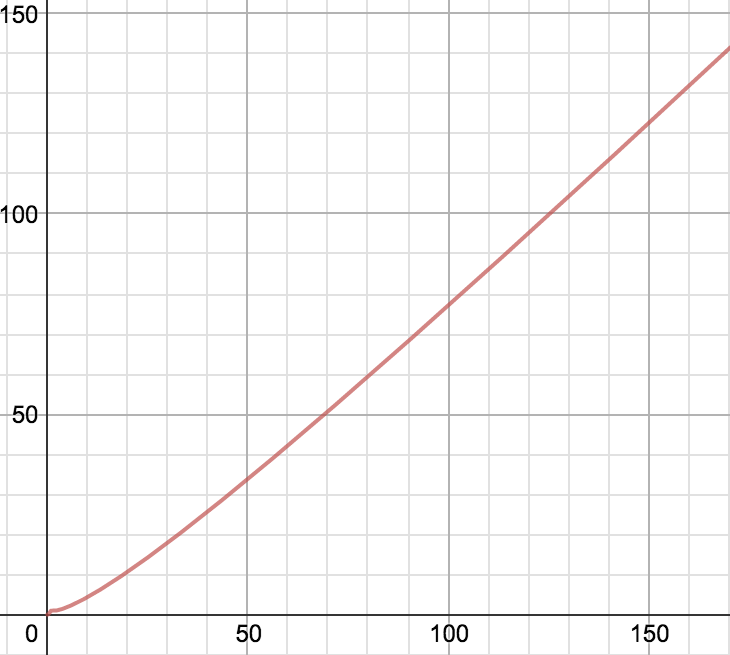
\includegraphics[width=350px,height=350px]{Equ5}\]
Note: Horizontal axis denotes $n$, vertical axis denotes possible matrices algorithm must test. As $n$ gets large, $(5)$ begins to resemble a linear function. This function hosts points including $(500, 457)$ $(1000,946.64)$ $(10000,9905.48)$. These points where $n$ is large support the notion that this function increases close to linearly.

\newpage
\section{\\Algorithm Pseudocode} \label{App: Appendix B}
\begin{algorithm}
\caption{Algorithm for Determining Isomorphism}
\begin{algorithmic}[1]

\Procedure{FindIso}{}
\State $A,A' \gets \text{Store matrix } A,A'$
\State $n \gets \text{length of A}$

\ForAll{$0\leq a,b<n$}
\State $A^*[a][b] \gets A[a][b] \oplus A'[b][a]$
\EndFor

\State $a,k \gets 0$
\State $A\sigma \gets \text{null values}$

\While{$a < n$}

\ForAll{$k \leq i \leq n$} \label{mainLoop}
\If{$A^*[a][i] == 0$}
$k = i$
\State \textbf{break}
\EndIf
\EndFor

\State $isIso \gets true$
\If{$A\sigma_{[a]} \neq A_{[k]} || A\sigma_{(a)} \neq A'_{(k)}$} \Comment{Testing only defined values in $A\sigma$}
\State $isIso \gets false$
\Else
\State $A\sigma_{[a]} = A_{[k]}, A\sigma_{(a)} = A'_{(k)}$
\State $a \gets a + 1$
\State $k \gets 0$
\EndIf

\If{$isIso==false \text{ and } k<n$}
\State $k \gets k+1$

\ElsIf{$k == n$}
\State $a \gets a-1$
\State $k \gets \text{ k value for previous row}+1$
\State $A\sigma \gets \text{ previous value of } A\sigma$
\Else
\State $a \gets a + 1$
\State $k \gets 0$
\EndIf
\EndWhile

\EndProcedure
\end{algorithmic}
\end{algorithm}

\newpage
\section{\\Python Implementation} \label{App: Appendix C}
\singlespace
\lstinputlisting[language=Python, basicstyle=\small]{AlgorithmTester.py}

\begin{table}[b!]
\begin{tabularx}{\textwidth}{@{} Y Y Y @{}} % use 'Y' for first column
\toprule
Example Input A & Example Input A' & Output \\
\midrule
\textbf{GraphArrayA.txt}\newline
0111\newline
1010\newline
1101\newline
1010 & 
\textbf{GraphArrayAPrime.txt}
0111\newline
1001\newline
1001\newline
1110 & 
Final Isomorphism:
[['0', '1', '1', '1'], ['1', '0', '1', '0'], ['1', '0', '1', '0'], ['1', '1', '0', '1']]\newline
Permutation List:
[0, 1, 3, 2] \\ \addlinespace
\bottomrule
\end{tabularx}
\caption{Expected Results} 
\label{table:nonlin}
\end{table}

\doublespace

\newpage
\begin{thebibliography}{9}
\bibitem{1}
  Frank Gaitan and Lane Clark,
  \emph{Graph isomorphism and adiabatic quantum computing},
  Laboratory for Physical Sciences, Maryland;
  Department of Mathematics, Southern Illinois University,
  2014.

\bibitem{2}
  Helen M. Grindley, Peter J. Artymiuk, David W. Rice, Peter Willett,
  \emph{Identification of Tertiary Structure Resemblance in Proteins Using a Maximal Common Subgraph Isomorphism Algorithm},
  Krebs Institute for Biomolecular Research Departments of Information Studies and of Molecular Biology and Biotechnology University of Sheffield, Western Bank, Sheffield
  2002.

\bibitem{3}
  P. Foggia, C.Sansone, M. Vento,
  \emph{A Performance Comparison of Five Algorithms for Graph Isomorphism},
  Dipartimento di Informatica e Sistemistica Via Claudio, Italy.

\bibitem{4}
  J.D. Schaffer, ed., Morgan Kaufmann,
  \emph{Using genetic algorithms to solve NP-complete problems},
  Los Altus, CA.
  1989.
  
  \bibitem{5}
   E. M. Luks,
  \emph{Isomorphism of Graphs of bounded valence can be tested in polynomial time},
  Journal of Computer System Science,
  1982.

 \bibitem{6}
   B. T. Messmer,
  \emph{Efficient Graph Matching Algorithms for Preprocessed Model Graphs},
  Inst. of Comp. Science and Appl. Mathematics, University of Bern,
  1996.
  
   \bibitem{7}
   Laszlo Babai,	
Eugene M. Luks,
  \emph{Canonical labeling of graphs},
  Proceedings of the fifteenth annual ACM symposium on Theory of computing, Pages 171-183, New York, USA,
  1983.
  
  \bibitem{8}
  Lov K. Grover,
  \emph{A fast quantum mechanical algorithm for database search},
  Proceedings, 28th Annual ACM Symposium on the Theory of Computing (STOC), May 1996, pages  212-219,
  1996.
  
\end{thebibliography}

\end{document}




  